\subsubsection{subfunction-oeSendHospitalInfo}

\label{RE-use-case-oeSendHospitalInfo}


send selected information to near hospitals		  


\begin{usecase}
  \addheading{Use-Case Description}
  \addsingletwocolumnrow{Name}{oeSendHospitalInfo}
  \addsingletwocolumnrow{Scope}{system}
  \addsingletwocolumnrow{Level}{subfunction}
  
\addrowheading{Parameters}
\addnumberedsinglerow{AdtHospitalInfo: dtHospitalInfo}{The selected information to the hospitals}
\addnumberedsinglerow{AdtCrisisID: dtCrisisID}{The crisis that the information belongs to}

\addrowheading{Primary actor(s)}
\addnumberedsinglerow{}{\msrcode{actCoordinator[active]}}


\addrowheading{Secondary actor(s)}
\addnumberedsinglerow{}{\msrcode{actHospital[passive, multiple]}}

\addrowheading{Goal(s) description}
\addsinglerow{send selected information to near hospitals}

\addrowheading{Protocol condition(s)}
\addnumberedsinglerow{}{The coordinator is already logged in
}
\addnumberedsinglerow{}{The system is already initialized
}

\addrowheading{Pre-condition(s)}
\addnumberedsinglerow{}{Exists a crisis that is being handling by this coordinator
}

\addrowheading{Main post-condition(s)}
\addnumberedsinglerow{}{The system sends information to near hospitals
}

\addrowheading{Additional Information}
\addsinglerow{
none
}

\end{usecase} 

Figure \ref{fig:lu.uni.lassy.excalibur.examples.icrash-RE-UCD-uc-oeSendHospitalInfo}
The coordinator send the selected information to near hospitals

\begin{figure}[htbp]
\begin{center}

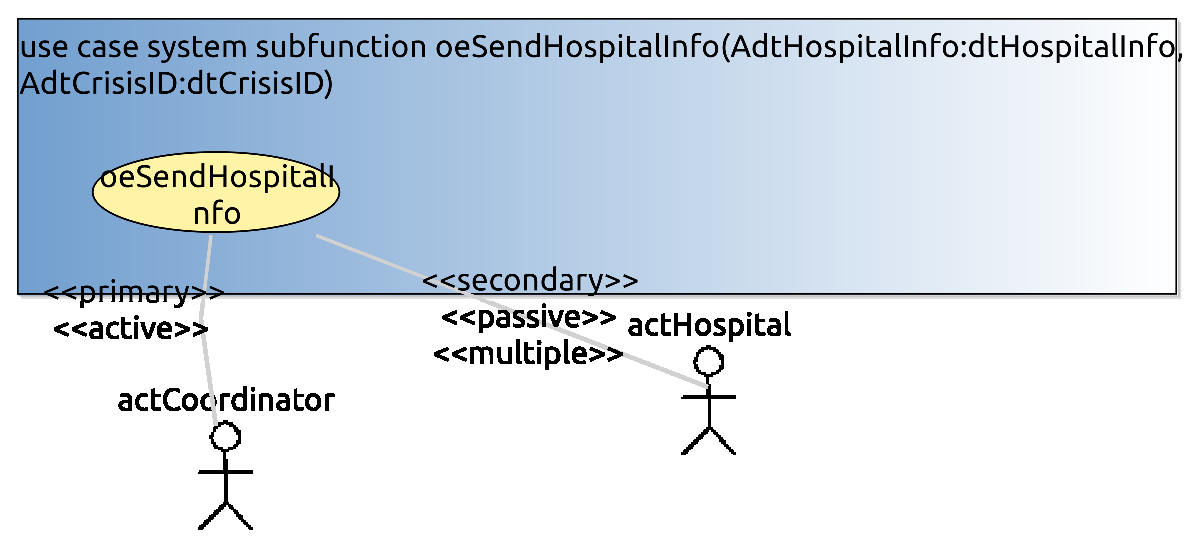
\includegraphics[
angle=0
]{./images-report-gen/usecase-model/subfunction/uc-oeSendHospitalInfo.eps}
\end{center}
\caption[lu.uni.lassy.excalibur.examples.icrash Use Case Diagram: uc-oeSendHospitalInfo]{}
\label{fig:lu.uni.lassy.excalibur.examples.icrash-RE-UCD-uc-oeSendHospitalInfo}
\end{figure}
\vspace{0.5cm}
